\newpage
\section{Rozproszone uczenie na urządzeniu końcowym}


\paragraph{Federated Learning}

Problemy odpowiednie do zastosowania federated learningu moją następujące właściwości:

1) Trening na rzeczywistych danych gromadzonych na urządzniach mobilnych dają znaczą przewagę
nad treningiem na ogólno dostępnych danych proxy dostępnych w centrach danych.

2) Te dane są prywatne albo są zbyt duże do przetrzywywnia ich w centrach danych

3) Dla zadań nadzorowanych, etykiety danych powstają samoistnie z interakcji użytkownika z użrządzeniem.



\paragraph{Optymalizacja}

Algorytmy optymalizacji mogące być sastosowane do optymalizajic na urządzniach IoT mają kilka cech wyróżniających je od znanych już algorytmów rozporoszonej optymalizacji:
\begin{itemize}

\item \textbf{Non-IID} Dane trenujące on danym urządzniu są zazwyczaj zależne od konkretnego użytkownika i dlatego lokalny zbiór danych zebrany na dowolnym urządzeniu nie będzie reprezentatywny w stosunku do dystrybucji całej populacji
\item \textbf{Niezbalansowany} Podobnie, niektórzy urzytkownicy będą o wiele częściej korzystali z aplikacji aparatu niż inni, co będzie prowadziło do różnic w wielkości zebranych lokalnych zbiorów  danych trenujących.
\item \textbf{Masywnie rozporszony} Spodziewa się, że liczba finalnych użytkowników biorąca udział w optymalizacji będzie większa niż średnia liczba przykładów trenujących przypadająca na jednego klienta.
\item \textbf{Ograniczona komunikacja} Urządznia IoT są pomimo założenia, że mają dostęp do
internetu mogą być ograniczone wolnym albo kosztownym łączem sieciowym.
\end{itemize}

W tej pracy główna uwaga zostanie poświęcona na rozwiązanie doprowadznie systemu do działania w środowisku danych Non-IID oraz ograniczonej komunkiacji.

\subsection{Implementacja}

  \begin{polishalgorithm}[t]
    \begin{algorithmic}
    \SUB{Server executes:}
      \STATE{} initialize $w_0$
      \FOR{each round $t = 1, 2, \dots$}
        \STATE{} $m \leftarrow \max(\clientfrac\cdot K, 1)$
        \STATE{} $S_t \leftarrow$ (random set of $m$ clients)
        \FOR{each client $k \in S_t$ \textbf{in parallel}}
          \STATE{} $w_{t+1}^k \leftarrow \text{ClientUpdate}(k, w_t)$ 
        \ENDFOR{}
        \STATE{} $w_{t+1} \leftarrow \sum_{k=1}^\nc \frac{n_k}{n} w_{t+1}^k$
      \ENDFOR{}
      \STATE{}
    
    \SUB{ClientUpdate ($k, w$):}\ \ \  // \emph{Run on client $k$}
      \STATE{} $\mathcal{B} \leftarrow$ (split $\pp_k$ into batches of size $\lbs$)
      \FOR{each local epoch $i$ from $1$ to $\lepochs$}
        \FOR{batch $b \in \mathcal{B}$}
          \STATE{} $w \leftarrow w - \eta \grad \loss(w; b)$
        \ENDFOR{}
    \ENDFOR{}
    \STATE{} return $w$ to server
    \end{algorithmic}
    \mycaptionof{algorithm}{\fedavglong. The $\nc$
      clients are indexed by $k$; $\lbs$ is the local minibatch size,
      $\lepochs$ is the number of local epochs, and $\eta$ is the learning
      rate.}\label{alg:fedavg}
    \end{polishalgorithm}


  Algorytm~\ref{alg:fedavg} opisany został zaimplementowany w języku Python. Do implementacji modeli
  neuronowych i algorytmów uczących został wykorzystany framework
  PyTorch~\cite{paszke2017automatic}. Poprawność implementacji została sprawdzona na zadaniu klasyfikacji obrazów wykorzystując prostą sieć konwolucyją oraz popularny zbiór danych CIFAR10. 

  \paragraph{Sieć konwolucyjna}

  Jako obiekt treningu omawianego algorytmu zastała użyta niewielka sieć neuronowa zawierająca
  dwie warstwy konwolucyjne z filtrami o szerokości 5x5 (pierwsza z 32 kanałami, druga z 64, po
  każdej dodatkowa warstwa 2x2 max pooling), po których następuje dwuwarstowy percepron i na
  końcu wartswa przeształcenia liniowego, co daje w sumie \(10^6\) miliona parametrów. Model został modsumowany w tabeli 


  \paragraph{CIFAR10}

  CIFAR10 jest popularnym syntetycznym zbiorem danych. Zbiór danych składa się z \(\num{60000}\)
  kolorowych obrazów podzielonych na \(\num{10}\) klas, z \(\num{6000}\) obrazami przypadającymi
  na jedną klase. Zawarte są w nim obrazy o szerokości i wyskości 32 pikseli. Standordowo zbiór
  dzieli się na dwa zbalansowane klasowo podzbiory: testowy i trenigowy zawierających odpowiednio
  \(10000\) i \(50000\) oetykietowanych przykładów. Na rysunku~\ref{fig:cifar10_example} znajduje się 10 losowo wybranych obrazów, dla każdej z 10 klas.

  \begin{figure}[t]
    \centering
    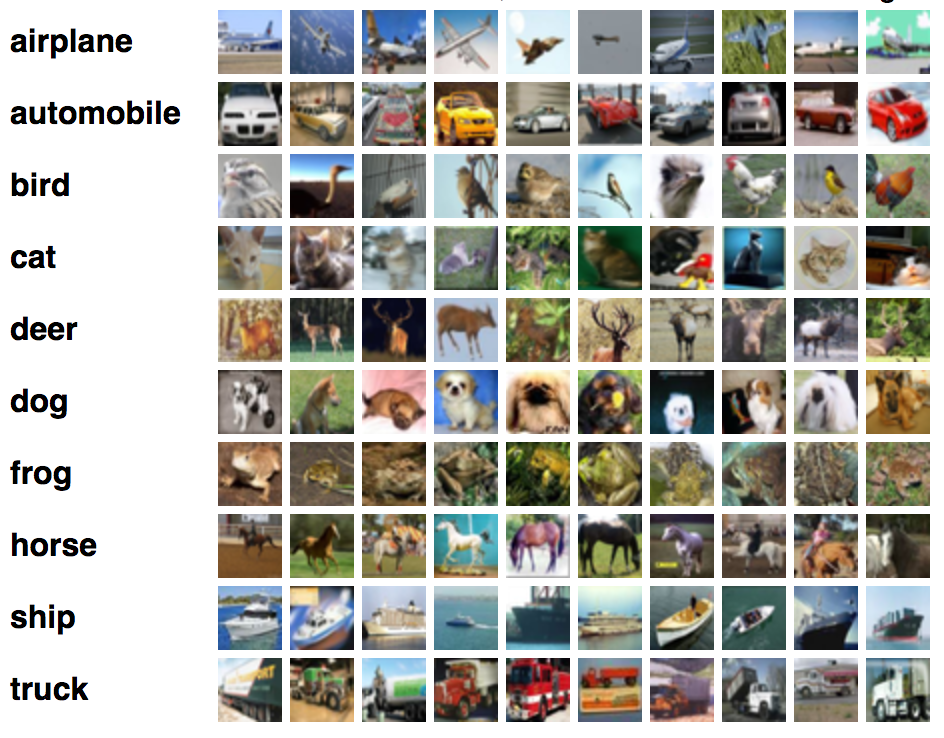
\includegraphics[width=1.0\textwidth]{img/cifar10_example.png}
    \mycaptionof{figure}{10 przykładowych obrazów dla każdej z \(\num{10}\) klas zbioru CIFAR10}
    \label{fig:cifar10_example}
  \end{figure}

  \paragraph{Protokół treningowy}

  Do sprawdzenia poprawności implementacji została zaimplementowana procedura treningowa wzorowana
  na~\cite{mcmahan2016communicationefficient}. Zbiór trengowy został podzielony pomiędzy 100 użytkowników tak żeby każdy zawierał po 500 przykładów trenujących. Z powodu braku naturalnego podziału danych na tak dużą liczbę klientów rozważany jest tutaj nieco mnie wymagający przypadek, w którym dane każdego użytkowanika są zbalansowane oraz IID.

  Naszym celem była maksymalizacja dokładności z jaką model klasyfikował obrazy pochodzące ze
  zbioru testowego. Badanie jakości końcowego modelu globalengo odbywało się już nie w sposób
  rozproszony, a na serwerze stosując cały dostępny zbiór testowy.

  Obrazy uległy standardowemu preprocessingu, który się składał z losowemu obcinanu obrazów do wielkości 24x24 pikselu, loswemu odbiciu lustrzanemu oraz standardowej normalizacji.

  Zaimplementowany algorym został porównany do standardowego algorytmu SGD.



  \paragraph{Ewaluacja}